\documentclass[11pt]{article}

\usepackage[a4paper, margin=2.3cm]{geometry}
\usepackage{graphicx}
\usepackage{setspace}
\usepackage{amsmath}
\usepackage{parskip}
\usepackage{float}
\usepackage{booktabs}
\usepackage{caption}
\usepackage{microtype}

\onehalfspacing
\graphicspath{{figures_fp/}{../figures/}}

% S-prefix for supplementary numbering
\renewcommand{\thefigure}{S\arabic{figure}}
\renewcommand{\thetable}{S\arabic{table}}
\renewcommand{\thesection}{S\arabic{section}}

\begin{document}

\begin{center}
{\Large \textbf{Supplementary Information}}

\vspace{0.2cm}
Climate Controls on Runoff Across Hydroclimatic Regimes Using ERA5-Land and Machine Learning Analysis

\vspace{0.2cm}
\textit{Mariia Solodiankina, Shengli Zhu}
\end{center}

\vspace{0.6cm}

% =======================================================================
\section{Seasonal trend structure}

Sen's slope magnitudes for all four variables at annual and seasonal resolution are shown in Fig.~\ref{fig:s_trendheatmap}. The heatmap complements Table~2 of the main text by exposing the seasonal breakdown of each trend. Italy's evapotranspiration increase is dominated by summer (JJA, $+1.05$~mm~yr$^{-1}$), with smaller but significant contributions from winter ($+0.21$) and autumn ($+0.41$). Bangladesh's precipitation decline is concentrated in the core monsoon seasons -- spring ($-6.31$~mm~yr$^{-1}$) and summer ($-6.33$~mm~yr$^{-1}$) -- while winter and autumn show no significant change. Saudi warming is broadly distributed but strongest in autumn ($+0.05$~$^\circ$C~yr$^{-1}$) and summer ($+0.04$).

\begin{figure}[H]
    \centering
    
\includegraphics[width=\linewidth]{fig07_trend_heatmap.png}
    \caption{Mann--Kendall/Sen's slope trend magnitudes for precipitation, evapotranspiration, runoff, and temperature, by country and season (1950--2025). Asterisks denote statistical significance at $\alpha = 0.05$.}
    \label{fig:s_trendheatmap}
\end{figure}

% =======================================================================
\section{Full annual SHAP feature distributions}

The bar chart in Fig.~5 of the main text summarises SHAP contributions by their mean absolute value, but hides the direction and spread of individual contributions. Figure~\ref{fig:s_beeswarm} shows the full SHAP distribution for every feature. High precipitation values systematically push the prediction up in all three countries, while in Italy high soil temperature values pull the prediction down, in line with stronger evapotranspiration suppressing runoff under warm conditions.

\begin{figure}[H]
    \centering
    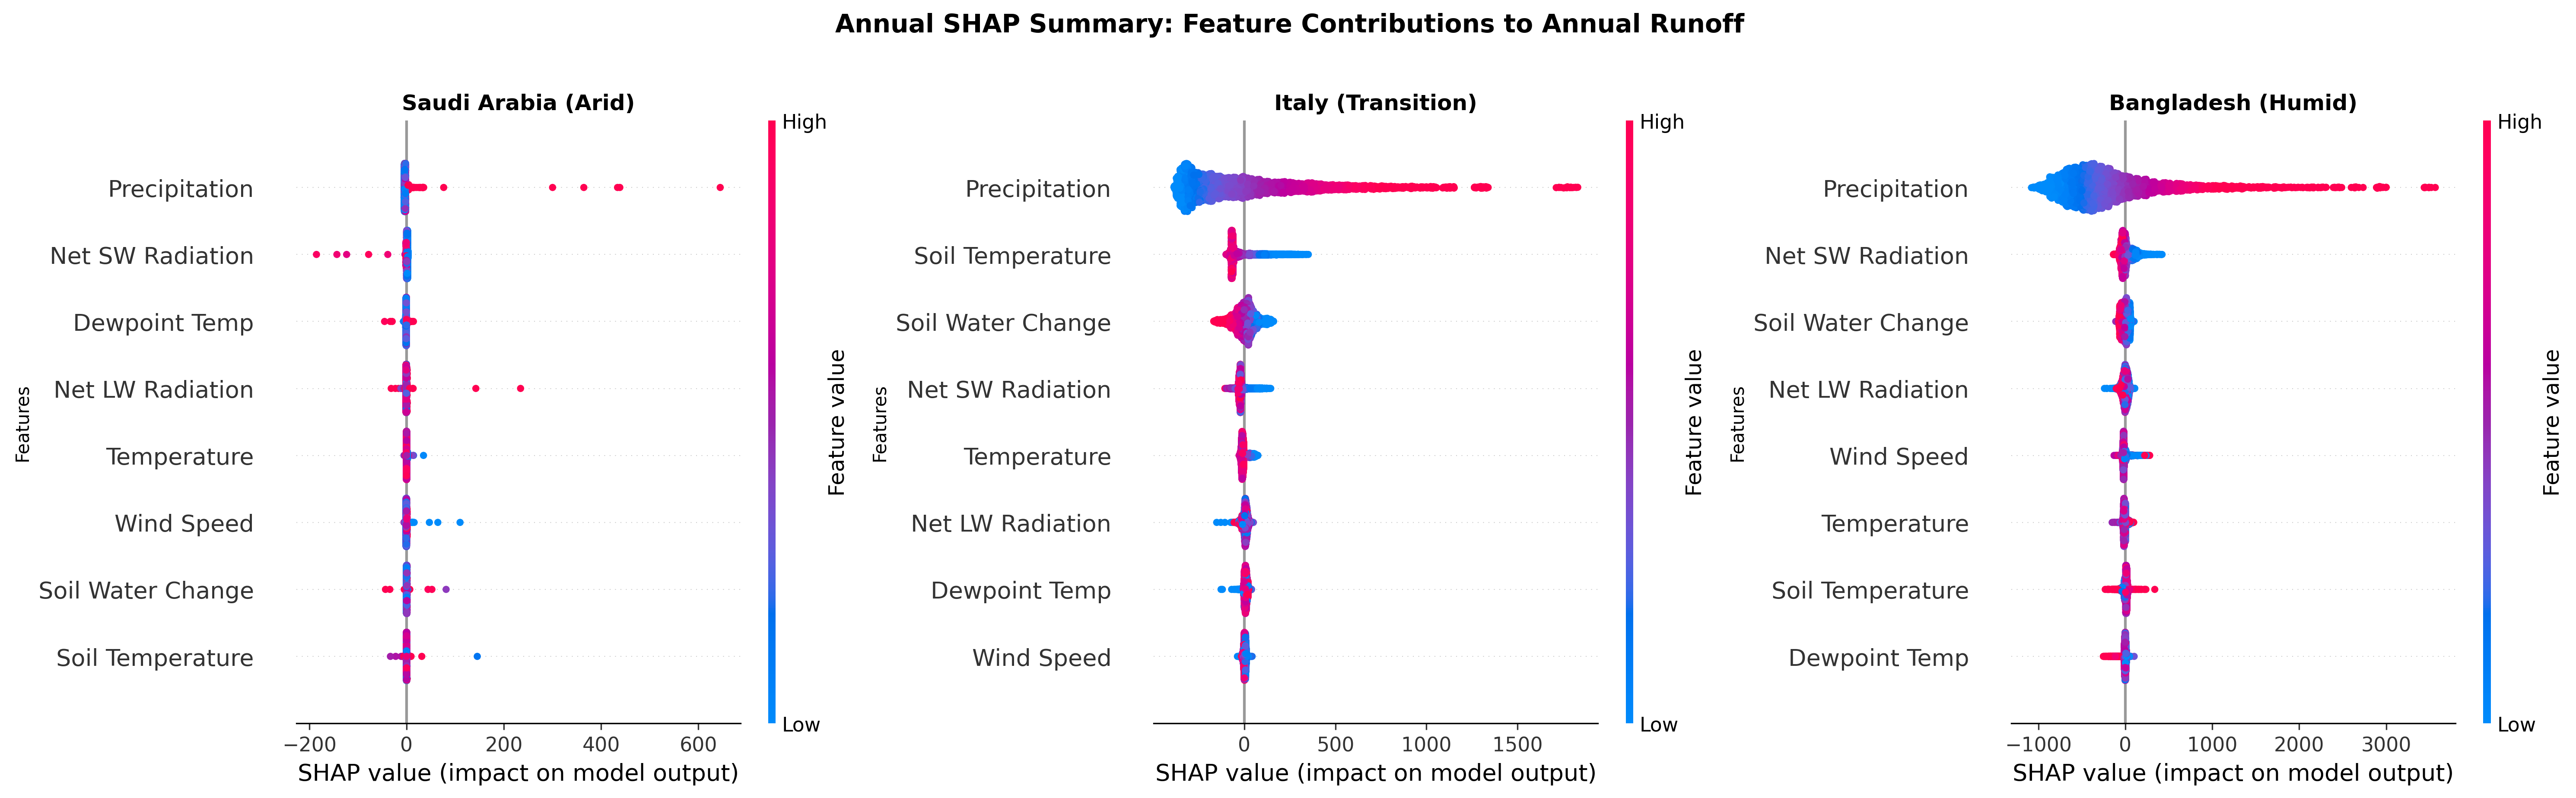
\includegraphics[width=\linewidth]{fig11b_annual_shap_summary.png}
    \caption{Annual SHAP beeswarm plots. Each point is one pixel-year from the test set. Horizontal position: SHAP contribution to predicted runoff; colour: raw feature value (red high, blue low).}
    \label{fig:s_beeswarm}
\end{figure}

% =======================================================================
\section{Temporal evolution of SHAP attributions}

Figure~\ref{fig:s_temporalshap} shows how the mean annual SHAP contribution of each feature has evolved between 1950 and 2025. Year-to-year variability is dominated by precipitation in all three countries, with the largest swings in Bangladesh during strong monsoon years in the 1970s and 1990s. In Italy, a mild declining trend in the precipitation SHAP contribution after 2000 mirrors the rising evapotranspiration reported in the main text. Saudi Arabia shows no coherent temporal structure beyond the first decade, in line with the low predictability of the arid-zone model.

\begin{figure}[H]
    \centering
    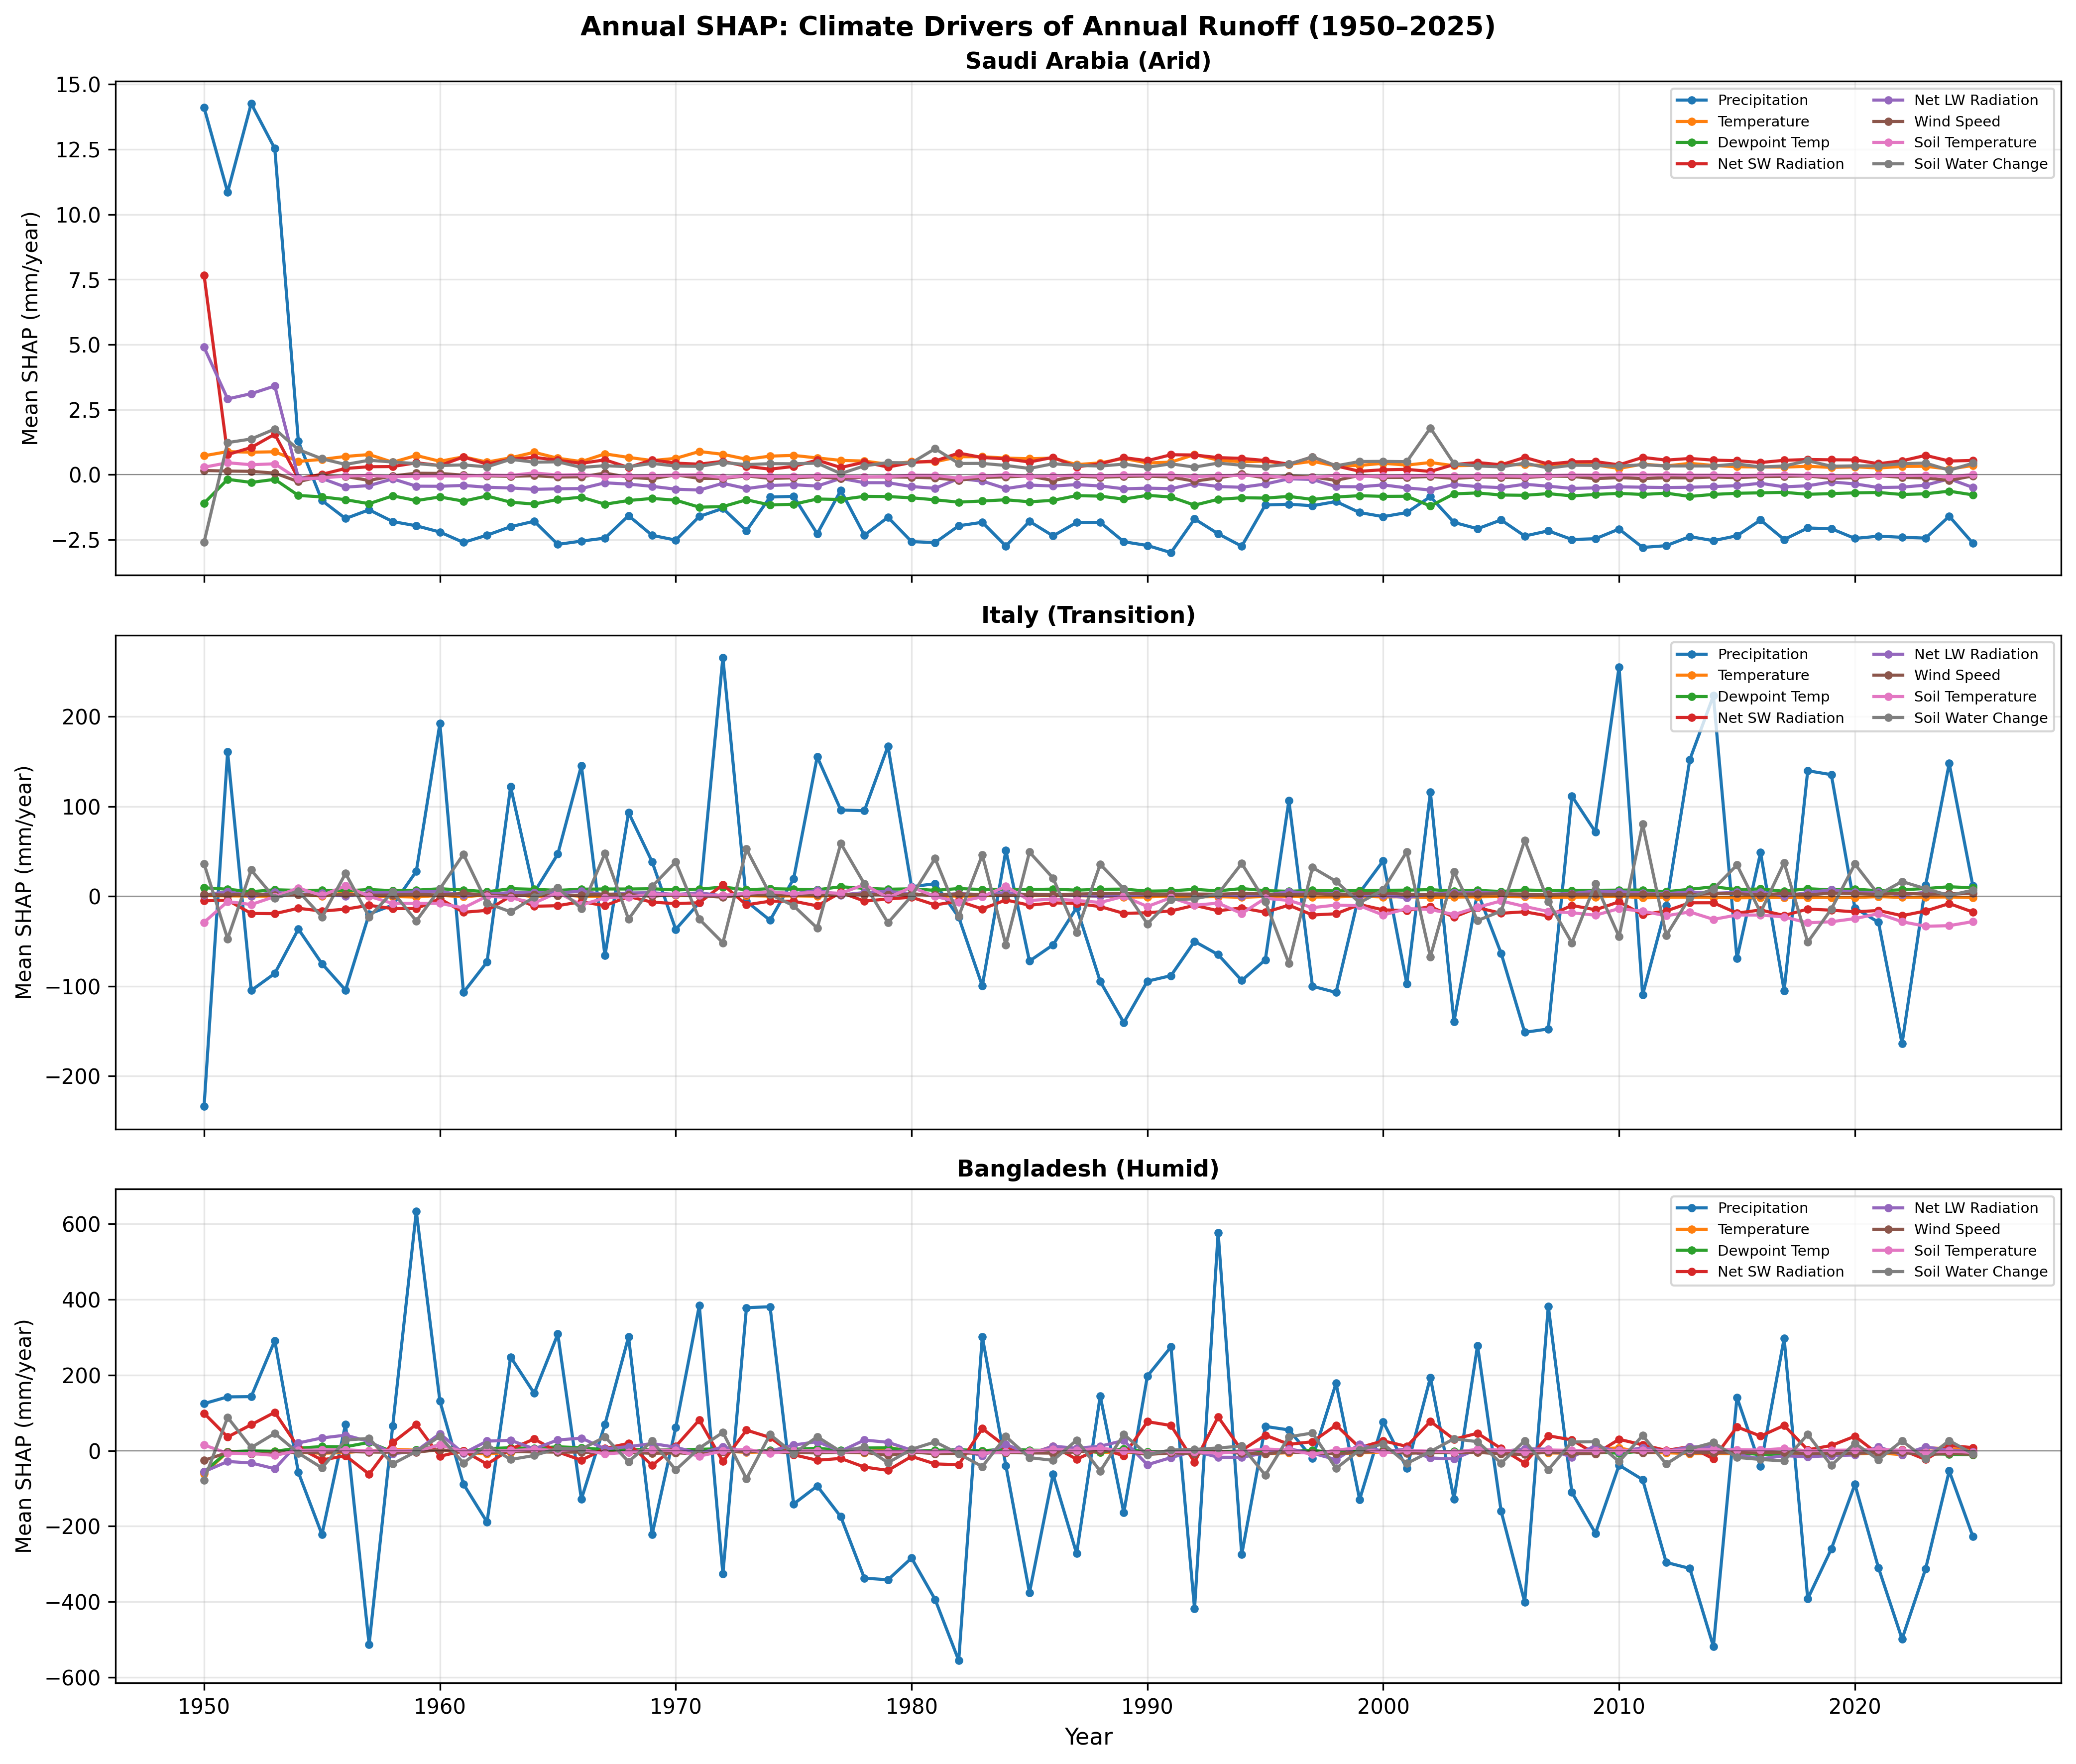
\includegraphics[width=\linewidth]{fig10b_annual_shap_temporal.png}
    \caption{Annual mean SHAP contribution per feature, 1950--2025, for each country. One marker per calendar year, no smoothing applied.}
    \label{fig:s_temporalshap}
\end{figure}

% =======================================================================
\section{Monthly-scale models: justifying the annual focus}

In addition to the annual model used in the main text, we trained parallel monthly XGBoost models on pixel-month records. Their performance and SHAP rankings explain why we chose the annual model for physical interpretation.

The monthly model performs markedly worse than the annual model in the hyper-arid regime ($R^2 = 0.36$ vs.\ 0.59 for Saudi Arabia) and exhibits a seasonality-driven attribution anomaly. In Italy the monthly model ranks soil temperature as the top feature (mean $|\mathrm{SHAP}|$ $\sim$63~mm~month$^{-1}$), well above precipitation ($\sim$17~mm~month$^{-1}$). Monthly soil temperature here acts as a seasonal proxy: low winter values coincide with high runoff from snowmelt and low evapotranspiration, while high summer values coincide with suppressed runoff. The model uses this seasonal covariance as a predictive shortcut. Aggregating to annual resolution removes the within-year covariance and places precipitation unambiguously first in every country. Monthly SHAP results are useful for diagnosing the model's internal structure but should not be used as a basis for physical attribution, which is why the main text reports only annual results.

\begin{figure}[H]
    \centering
    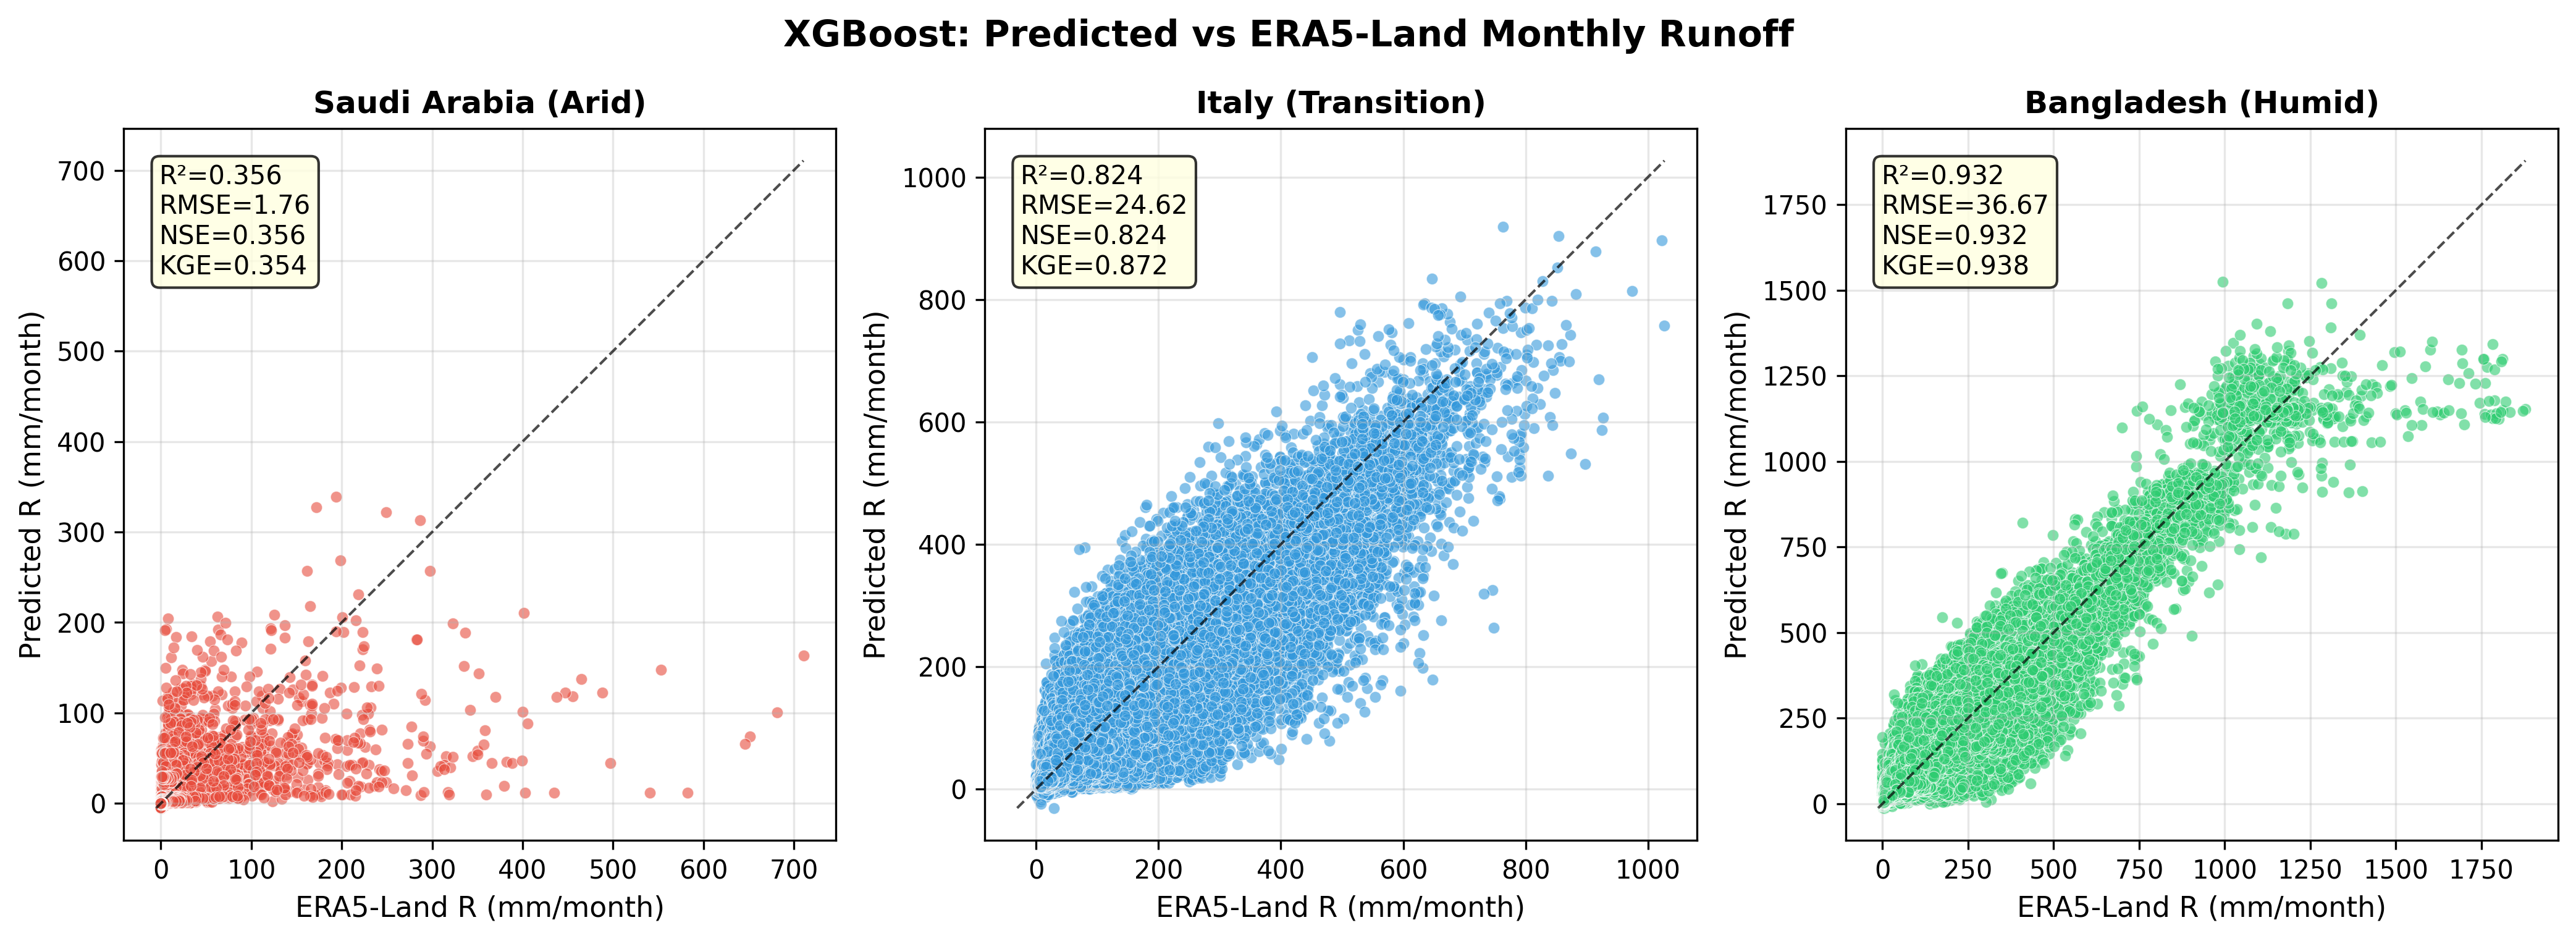
\includegraphics[width=\linewidth]{fig09_predicted_vs_observed.png}
    \caption{Monthly XGBoost predictions versus ERA5-Land reanalysis runoff on the held-out test period (2005--2025). Compare with Fig.~4 of the main text (annual model).}
    \label{fig:s_monthly_pvo}
\end{figure}

\begin{figure}[H]
    \centering
    
\includegraphics[width=\linewidth]{fig12_shap_bar_comparison.png}
    \caption{Monthly-model mean absolute SHAP values. Note that soil temperature exceeds precipitation in Italy, an artefact of strong seasonal covariance at the monthly scale.}
    \label{fig:s_monthly_bar}
\end{figure}

\end{document}
